
%(BEGIN_QUESTION)
% Copyright 2012, Tony R. Kuphaldt, released under the Creative Commons Attribution License (v 1.0)
% This means you may do almost anything with this work of mine, so long as you give me proper credit

Suppose you were given a conductivity transmitter and a toroidal probe that is supposed to go along with it:

$$\includegraphics[width=15.5cm]{i01126x01.eps}$$

Your task is two-fold.  First, explain how you can identify which leads on the probe connect to which terminals on the transmitter using nothing but a multimeter (hint: the two coils inside the toroidal probe are supposed to be identical to each other).  Second, describe a way to ``dry-test'' this probe once it's connected to the transmitter (i.e. without using any liquid to dip the probe in).  Your proposed test must be able to simulate varying degrees of conductivity, rather than being an ``all-or-nothing'' type of test.

\underbar{file i01126}
%(END_QUESTION)





%(BEGIN_ANSWER)

5 points for explanation of wire identity; 5 points for description of dry test:

\vskip 10pt

An ohmmeter would be a good tool to use when identifying probe wires.  Checking for resistance (continuity), you should measure low resistance (good continuity) between two wires connecting to a coil.

\vskip 10pt

Once the probe has been connected to the transmitter, you may test it by providing an electrically conductive path through the center hole (the ``donut hole'') of the probe, just as conductive water will provide a circuitous path for current through this hole.  A jumper wire connected to a variable resistor will suffice.  Note: {\it it is essential that students understand this must be a \underbar{loop} of conductive material through the center of the toroids, not just a piece of conductive material.}  Do not award any points for a ``dry test'' based simply on placing a piece of conductive material in the hole of the probe!

%(END_ANSWER)





%(BEGIN_NOTES)

{\bf This question is intended for exams only and not worksheets!}.

%(END_NOTES)


